\documentclass{scrartcl}
\usepackage[T1]{fontenc}
\usepackage[utf8]{inputenc}
\usepackage[ngerman]{babel}
\usepackage{amsmath,amssymb}
\usepackage{enumerate}
\usepackage{graphicx}

\begin{document}
\section*{Aufgaben zum Thema Graphen}
\begin{enumerate}[(1)]

\item Zeigen oder widerlegen Sie: Ein k\"urzester-Wege-Baum ist auch ein minimaler Spannbaum.

\item \begin{enumerate}[(a)]
\item Zeigen Sie: Dijkstra liefert bei negativen Kanten in gerichteten Graphen auch ohne negative Kreise im Allgemeinen ein falsches Ergebnis.
\item Geben Sie einen stark zusammenh\"angenden, gerichteten Graphen mit mindestens einer negativen Kante an, so dass Dijkstra f\"ur mindestens einen Startknoten ein korrektes Ergebnis liefert.
\item Warum funktioniert Dijkstra nicht auf zusammenh\"angenden, ungerichteten Graphen mit mindestens einer negativen Kante?
\end{enumerate}

\item Ein Graph G = (V,E) sei durch die folgende Adjazenzfelddarstellung gegeben:\\
\ \\
V := \begin{tabular}{|c|c|c|c|c|c|}
\hline 
1 & 3 & 4 & 6 & 9 & 11 \\ 
\hline 
\end{tabular}  \\
\ \\
E := \begin{tabular}{|c|c|c|c|c|c|c|c|c|c|c|}
\hline 
2 & 3 & 4 & 2 & 5 & 2 & 3 & 6 & 1 & 6 & 5 \\ 
\hline 
\end{tabular}\\
\begin{enumerate}[(a)]
	\item Zeichnen Sie den Graphen.
	\item Geben Sie den Graphen in Adjazenzlistendarstellung an.
	\item Welche dritte Möglichkeit zur Darstellung von Graphen wurde in der Vorlesung vorgestellt? Beschreiben Sie sie kurz und nennen Sie sowohl einen Vor- als auch einen Nachteil dieser Methode.
\end{enumerate} 

\item Wenden Sie die Algorithmen von Prim und Kruskal auf den folgenden Graphen an. Geben Sie dabei jeweils die Reihenfolge der betrachteten Kanten bzw. Knoten an.

\begin{figure}[h]
\centering
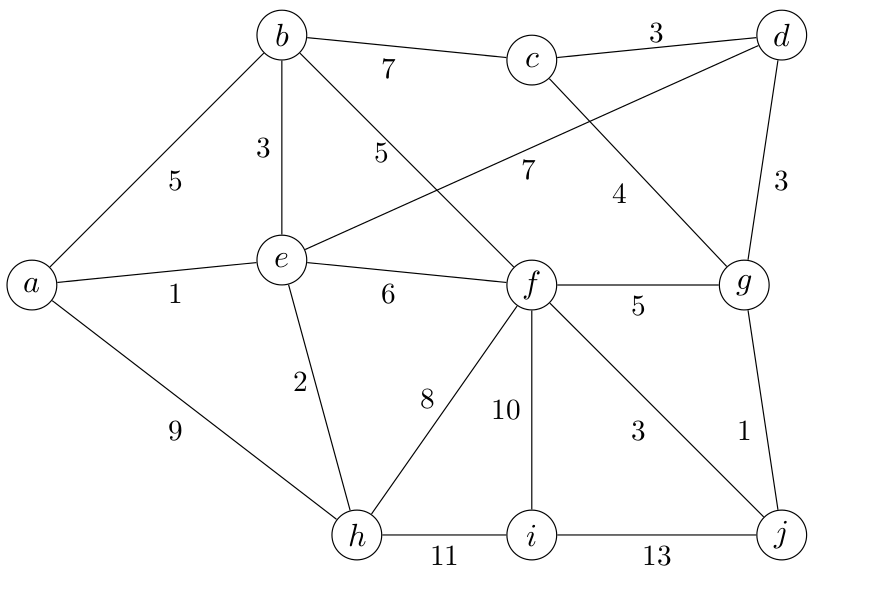
\includegraphics[width=0.66\textwidth]{mst_graph.png}
\end{figure}

\end{enumerate}

\end{document}
